\documentclass[10pt,twocolumn]{article}
\usepackage[letterpaper,margin=0.78in,columnsep=0.26in]{geometry}
\usepackage[T1]{fontenc}
\usepackage{lmodern,microtype,amsmath,amssymb,amsthm,booktabs,graphicx,array}
\usepackage[numbers,sort&compress]{natbib}
\usepackage{tikz}
\usetikzlibrary{arrows.meta,positioning}
\usepackage{xurl}
\usepackage[hidelinks]{hyperref}
\usepackage{fancyhdr,balance,caption}
\captionsetup{font=small,labelfont=bf}
\pagestyle{fancy}\fancyhf{}
\fancyhead[L]{\small Witness-CL v0.8}\fancyhead[R]{\small Development study, September 2026}
\fancyfoot[C]{\thepage}\setlength{\headheight}{14pt}
\setlength{\emergencystretch}{1.5em}
\newtheorem{theorem}{Theorem}
\newtheorem{proposition}[theorem]{Proposition}
\newcommand{\E}{\mathbb E}
\title{\vspace{-1.2em}\textbf{Witness-CL: Checked Executable Memories\\and a Failed Online-Abstraction Pilot}}
\author{Samuel Mausberg\\\small AI-assisted research draft; author review and independent replication pending}
\date{}
\hypersetup{pdftitle={Witness-CL: Checked Executable Memories and a Failed Online-Abstraction Pilot},pdfauthor={Samuel Mausberg},pdfsubject={Typed SQL fragments, experience provenance, competence failures, and limits of retention guarantees}}
\begin{document}
\raggedbottom
\maketitle
\begin{abstract}
Can an online agent discover executable abstractions from its own experience,
reuse them on new compositional tasks without task identifiers or an enumerated
semantic feature library, reduce interaction relative to full-history and
evolving-memory controls, and retain prior competence? We implement a bounded
SQL agent intended to test that conjunction. Its model may synthesize a new
parameterized relation after a correct episode; admission requires a charged
execution that reconstructs its own observed scalar result. A typed compiler
supports rebinding and a new outer SELECT, with exact prepared-request properties
checked in Lean. A frozen six-arm development pilot uses one local Qwen3-4B
backbone, opaque schemas, queryable business documentation, fresh database rows,
and separate frozen evaluation panels. All six arms score zero on the eight
warm questions. Neither executable-memory arm admits or uses an abstraction.
The run therefore fails the predeclared competence prerequisites and does not
establish the target claim. We report the complete cost and outcome record,
identify transcript-level failure mechanisms, and distinguish compiler correctness,
finite reconstruction evidence, observed transfer and behavioral retention.
\end{abstract}

\section{Question and scope}
The intended contribution is a conjunction of discovery, transfer, efficiency
and preservation. Each is necessary. A smaller prompt does not establish lower
interaction at equal accuracy; a correct answer does not establish use of a
learned abstraction; and unchanged failure does not establish retention of a
useful capability. This report makes the attempted mechanism concrete and records
why its first model pilot does not satisfy that conjunction.

CL-Bench evaluates learning across stateful domains and reports a strong raw-history
ICL baseline relative to dedicated memory systems~\cite{clbench}. AgentCL constructs
streams with reusable components and separates transfer from performance on less
structured task streams~\cite{agentcl}. These motivate both mandatory history
controls and an explicit audit of task relationships. This custom SQLite study
is not an execution of either benchmark and gives no native benchmark score.

The implementation removes two major restrictions of the preceding Witness-CL
experiment: the learner receives neither authentic report IDs nor an enumerated
84-monomial feature library. Instead, a language model writes ordinary SQL from
public instructions and its own tool observations. SQL syntax, the action API,
the pretrained model, and the bounded memory representation remain inductive
biases. Removing a semantic feature list does not mean removing every grammar
or proving that the foundation model has never encountered similar programs.

The new evidence consists of a complete executable pipeline, 12 additional
Lean statements, differential compiler fixtures, independent saved-data replay,
and a negative development pilot. The previous v7 empirical result and its
source freeze are preserved separately; neither its positive within-family
transfer contrast nor its structural routing guarantee is relabeled as a result
for this agent.

\section{Environment and information boundary}
An episode supplies a natural-language scalar question and SQLite CREATE
statements with randomized table and column names. Four data relations represent
orders, customer profiles, refunds and shipments. A queryable \texttt{catalog}
table documents column meanings, monetary units, missing-value conventions,
profile multiplicity and the rule identifying current profiles. Meaning is
therefore discoverable by legal interaction. It is not supplied through a
hidden family label or a model-visible oracle program.

Each database has 32 orders, eight customers and bounded related records.
Each ordinary and distinct panel fixture has independently generated rows;
the same fixed fresh-old fixtures are reused in both retention measurements.
A SELECT returns
at most 50 rows and is subject to cell, byte, VM-step and time limits. All
attempts count, including failed SQL, malformed actions, applicability checks,
fragment execution and post-answer reconstruction. Each episode permits eight
attempts and ten model action calls. The host rejects writes, attachments,
extensions, file functions and recursive CTEs. The model emits structured text
and has no Python, shell or network tool authority.

Correctness feedback is one binary outcome after a submitted finite numeric
answer. The model never receives the numerical target. The evaluator records
reference information only after model interaction is finished. During ordinary
learning, an unused query allowance may support a reconstruction check after
scoring; this cannot revise the scored answer. Evaluation panels disable that
learning path and cannot update cross-episode memory. The interface is a
restricted executor for model-generated SQL, not an operating-system isolation
claim against arbitrary host-process introspection.

\subsection{Composition and retention}
Each stream has eight warm questions, eight middle questions that recombine
previously required relations, and eight later questions involving more complex
operations. The middle block includes profile-conditioned net value, refund/gross
ratios, grouped extrema and differences of conditional averages. Its required
target structures differ from the warm questions after literal normalization.
Question 17 introduces shipment delivery; question 18 adds latest-shipment timing.
The late block is reported separately because these operations are new learning
requirements, not pure transfer of already practiced skills.

The composition audit uses normalized target syntax and manually specified
minimal semantic dependencies. It avoids raw SQL hashes that can differ merely
because of unused CTEs. This verifies opportunities in the task construction;
it does not prove arbitrary SQL inequivalence or show that a learner acquired
or used the annotated components. Correct transfer additionally requires a
traceable earlier learned relation, changed arguments or a new outer operation,
and a correct result causally dependent on that relation.

Eight old questions keep the initial public instructions, schema and conventions,
with independent fresh rows. The same fixed fresh-old panel runs with memory
frozen after warm learning and after all ordinary learning. Eight final questions
then test new compositions with final memory frozen. In the actual development
fixture seven of eight old targets differ from their corresponding warm targets.
Refunded-order count is structurally 22 because order $i$ has $i\bmod3$ refund
records. We retain this item in the declared endpoint and report it separately;
its answer can be cached. Fresh data alone does not guarantee a fresh answer.

Development and prospective heldout conventions use opposite parities of four
binary convention bits. Post-warm templates also differ. The name/data seed
function does not incorporate the split label, so a future evaluation must use
predeclared disjoint numeric seeds. No heldout model run was performed. The
observed pilot contains only the reusable condition; drift and nonreuse
conditions are implemented but have no measured result here.

\section{Experience-derived executable memory}
An ordinary successful episode may trigger one additional model call. The
proposal specifies a new SELECT relation, typed named literal bindings, an outer
SELECT over a CTE named \texttt{reused}, a description, and indices identifying
its own source query and applicability observation. The source must be a
successful scalar query consistent with the episode's confirmed answer. All
indices refer to the immutable pre-proposal prefix, preventing a model from
retroactively manufacturing its source evidence.

The host compiles the proposed relation and wrapper, then executes their
composition on the same database using one remaining SELECT attempt. Admission
requires a single finite numeric result within
$10^{-6}(1+|a|)$ of the witnessed answer $a$. This empirical comparison ignores
column labels; the applicability comparison below is stricter. The request,
result, attempt index, trace digest and proposal fields are recorded. A missing
witness, failed execution, invalid binding or mismatch prevents admission.
The prior answer remains scored even when its later proposal fails.

Up to 16 immutable entries are stored. Content overlap between the current
question and memory descriptions retrieves at most two entries. This router
uses no task identity, phase, evaluator recipe or hidden convention bit. A
\texttt{USE} action rebinds one relation. A \texttt{COMPOSE} action places it under
a new outer SELECT. Composition supports one learned inner relation and one
new wrapper, not arbitrary multi-library program synthesis.

Before checked reuse, the host executes the stored applicability query and
compares all returned columns and rows with its complete witnessed result.
A mismatch returns the observed evidence and permits ordinary solving. If this
check consumes the last allowed query, the fragment is not executed. The
unchecked arm omits this check to expose its potential benefit and cost.

\begin{figure*}[t]
\centering
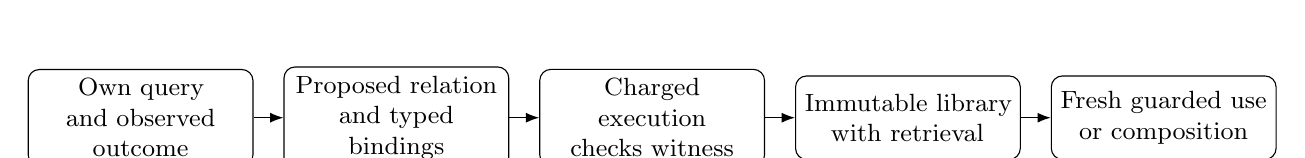
\begin{tikzpicture}[node distance=0.38cm,box/.style={draw,rounded corners,align=center,font=\small,text width=2.62cm,minimum height=1.06cm},>=Latex]
\node[box] (a) {Own query\\and observed outcome};
\node[box,right=of a] (b) {Proposed relation\\and typed bindings};
\node[box,right=of b] (c) {Charged execution\\checks witness};
\node[box,right=of c] (d) {Immutable library\\with retrieval};
\node[box,right=of d] (e) {Fresh guarded use\\or composition};
\draw[->] (a)--(b);\draw[->] (b)--(c);\draw[->] (c)--(d);\draw[->] (d)--(e);
\end{tikzpicture}
\caption{Implemented discovery path. Compiler contracts apply to prepared-request
construction. A passing reconstruction is finite evidence, not proof of future
semantic correctness. In the actual pilot neither fragment arm reached admission;
this diagram describes the implemented algorithm, not observed discovery.}
\label{fig:path}
\end{figure*}

\subsection{Why admission is insufficient}
A relation returning the already known scalar can reconstruct it perfectly.
A wrapper may ignore \texttt{reused} entirely. Neither demonstrates abstraction
or compositional transfer. Mutation and execution tests deliberately include
these cases: they may satisfy the finite witness check yet fail on fresh data.
The evidence standard therefore separates accepted reconstruction witnesses
from successful new-task uses. This is also why a zero answer that happens to
be correct without any query cannot supply a source-query witness.

Memory caps are explicit. A fragment has at most 32 Text/Hole parts, 4,096 SQL
bytes and an 8,192-byte serialized payload. A Text part may contain many SQL
syntax nodes: this is not a 32-node parsed-SQL bound. The active library cap is
65,536 bytes. FIFO eviction and failed routing can lose useful behavior.
Serialized retained history, descriptions, provenance and journals count toward
storage; exported audit files are reported separately and are not retrievable.

\section{What is formally established}
The added Lean module uses typed values, SQL text parts, parameter holes,
assignments and a fixed compiler. Python transports integers, finite binary64
values, text and null using SQLite bindings. Named values never substitute SQL
identifiers. Inner and outer parameter names are renamed into disjoint scopes,
including repeated names and quoted colons. The following statements summarize
the checked contracts; details and theorem inventory are in the repository.

\begin{theorem}[Captured-request identity]
For a fragment $f$ and its captured assignment $\theta_0$, binding $f$ at
$\theta_0$ and compiling under any later assignment yields exactly the captured
SQL text and parameter values. Supplying this identical request to the same
fixed executor function and database yields the identical modeled result.
\end{theorem}
\begin{proof}
Binding replaces each typed parameter occurrence with its captured value while
preserving text parts. Compilation concatenates the same text and occurrences.
Structural induction establishes the request identity; congruence of the fixed
executor gives the result identity. These are checked Lean equalities, not a
postulated SQL correctness theorem.
\end{proof}

Typed substitution also commutes with the compiler under the correspondingly
substituted assignment. Changing bound values cannot change SQL text, and
parameter-node renaming preserves transported values. The composition theorem
identifies compilation with the stated CTE expansion and its separated inner
and outer bindings. These statements cover the representation, not whether a
model-generated query expresses a user's intended computation.

\begin{proposition}[Conditional retention of the modeled fallback]
In the abstract answer-level guard operator, a failed or unavailable check
returns a supplied ordinary-policy answer. If every accepted protected
execution also produces that answer, this operator agrees pointwise with the
ordinary policy.
\end{proposition}
\begin{proof}
Split on the applicability decision. The rejecting branch is the ordinary
answer by definition. The accepting branch agrees by the stated premise.
\end{proof}

This operator is not a refinement proof of the model-driven fallback loop.
The implemented agent receives check feedback and resumes solving with a
changed prompt and reduced SELECT allowance; its resulting answer need not
equal the answer of an ordinary solver that never ran the check. The premise
is substantive and is not implied by observing a passing check.
The module gives counterexamples: observation of zero cannot identify scale
one versus scale 100, and a check that still passes after drift can accept one
when the correct answer becomes 100. Thus the construction cannot guarantee
unconditional preservation in arbitrary future environments. An immutable
library also does not force retrieval or later interpretation to be correct.

The complete repository now has 89 checked statements, including these 12 new
statements. The audit records standard logical dependencies and finds no custom
source axioms, proof placeholders or unexpected dependencies. A finite suite
compares 36 Lean-generated request cases with Python capture, rebinding,
composition and actual SQLite execution. It covers repeated parameters, quoted
colons, nulls, exact binary64 transport and SQL-shaped text values. These are
correspondence tests, not a machine-checked refinement of all Python or SQLite.

A \emph{compiler witness} preserves the captured proposed request exactly.
A \emph{learning witness} is the separately executed reconstruction of a prior
successful scalar result. No theorem equates the new proposed relation with
the original successful SQL on every database or future argument. Neither
successful discovery, interaction advantage, model quality nor the statistical
retention margin is proved in Lean.

\section{Frozen model pilot}
The development pilot was frozen before any database-task model call and
committed as \texttt{54cd9c8}. The official Qwen3-4B Q8\_0 weights, model-file
hash, llama.cpp revision, prompts, seven executed source files and protocol are
recorded. The backbone uses native 32,768-token context, one inference slot,
temperature zero, fixed seed 42 and thinking disabled. Solve outputs are capped
at 384 tokens and reflections at 1,024. This greedy setting differs from the
model card's non-thinking sampling recommendation~\cite{qwen3gguf}; the result
is specific to the frozen model/interface configuration, not a claim about
optimal Qwen performance. Weights are never updated.

Every request has an exact backend tokenization preflight. Its time, inference,
output usage and failures are recorded. No hidden retry, prompt truncation or
prompt-cache reuse is allowed. Each arm has the same 500,000 ordinary-token and
500,000 panel-token ceilings, respectively 280 and 260 model-call ceilings, and
the same episode SELECT allowance. The complete pilot has a 1,800-second global
ceiling including setup, solving, learning, checks, panels and incremental export.
Download, load and two transport-only preflights are separately reported setup.

The six arms are full history, content-retrieved complete episodes, evolving
natural-language insights, checked fragments, unchecked fragments and stateless.
All share the model and initial solving instructions. Full history retains every
own ordinary interaction without truncation. Retrieved episodes keep their full
backing archive but display two entries. Insights are revised by a charged
reflection after every ordinary episode, retaining at most 16 entries of at
most 512 characters each. That arm is a transparent evolving-memory control,
not a reproduction or strongest tuning of ExpeL or ACE.

The arm order rotates by scheduled question. A run has 24 ordinary and three
eight-question frozen panels, producing 288 arm-episodes across six arms.
The qualification rule requires at least six of eight warm answers correct
for both full-history and insight controls, at least six of eight fresh-old
answers before later learning for the proposed agent, and correctly traced
parameter reuse/composition. Failing that rule prevents a strong-control
superiority interpretation even if costs are fully accounted.

\section{Results and failure analysis}
\begin{table*}[t]
\centering\small
\begin{tabular}{lrrrrrr}
\toprule
Arm & Warm & Middle & Late & Old pre & Old post & Final \\
\midrule
Full history & 0/8 & 0/8 & 0/8 & 0/8 & 0/8 & 1/8 \\
Retrieved episodes & 0/8 & 1/8 & 0/8 & 0/8 & 0/8 & 2/8 \\
Evolving insights & 0/8 & 0/8 & 0/8 & 0/8 & 0/8 & 2/8 \\
Checked fragments & 0/8 & 1/8 & 0/8 & 0/8 & 0/8 & 2/8 \\
Unchecked fragments & 0/8 & 1/8 & 0/8 & 0/8 & 0/8 & 2/8 \\
Stateless & 0/8 & 0/8 & 0/8 & 0/8 & 0/8 & 2/8 \\
\bottomrule
\end{tabular}

\caption{Correct answers on every declared block of the single development
stream. Each cell is out of eight. Old pre/post use the same fresh fixtures
with memory frozen. Correlated questions are not independent replication units.
The full-history and insight warm qualification threshold is 6/8; both fail.}
\label{tab:acc}
\end{table*}
\begin{table*}[t]
\centering\small
\begin{tabular}{lrrrrrr}
\toprule
Arm & SELECTs & Calls & Input tok. & Output tok. & Model s & Peak KiB \\
\midrule
Full history & 52 & 100 & 621,930 & 2,897 & 219.4 & 36.4 \\
Retrieved episodes & 85 & 133 & 159,411 & 3,882 & 115.8 & 23.2 \\
Evolving insights & 11 & 83 & 61,027 & 5,011 & 82.0 & 4.4 \\
Checked fragments & 30 & 79 & 59,674 & 3,221 & 51.3 & 3.8 \\
Unchecked fragments & 30 & 79 & 59,674 & 3,221 & 48.7 & 3.8 \\
Stateless & 99 & 147 & 145,402 & 13,101 & 171.2 & 3.7 \\
\bottomrule
\end{tabular}

\caption{All recorded interaction and model costs across 48 episodes per arm,
including panels and charged learning calls. Model seconds include tokenization
and inference. Storage is the reported peak serialized retained state, not
process RAM or GPU memory. Low cost at low accuracy is not efficiency evidence.}
\label{tab:cost}
\end{table*}
Tables~\ref{tab:acc} and~\ref{tab:cost} report every declared block and total costs.
The complete pilot finishes in 690.13 seconds (11.50 minutes), within the
30-minute ceiling. It records 621 model calls, 1,107,118 input and 31,333 output
tokens, and 307 SELECT attempts. Of these attempts, 141 return SQL errors.
All 288 episode records pass independent replay, including 48 reference-case
checks and the exact frozen source map. No record has unknown model usage,
resource exhaustion or a runtime failure. Complete accounting does not imply
competence: there are only 14 correct answers in the entire six-arm grid,
and no accepted reconstruction witness or executable reuse.

The six raw trace files occupy 8,915,985 bytes, separately from learner memory.
Download and hash verification take 164.38 seconds, model loading 28.13 seconds,
and the two transport-only preflights use 481 tokens and 1.40 seconds including
tokenization and inference. These setup costs are excluded from the pilot clock
and are not hidden within a particular arm. The owned authenticated loopback
inference server was stopped after the completed pilot. No further model calls,
heldout runs or paid inference were performed for this report.


The failure occurs before useful abstraction learning. All six arms score
0/8 on warm questions. The checked and unchecked fragment arms end their
warm episodes by submitting zero without querying. Both later obtain one
correct ordinary zero answer without an observed query. Each proposes a
fragment afterward, but admission rejects it for lacking a source witness.
No fragment is admitted, rebound or composed in this pilot. All 14 correct
scored answers equal zero; none uses an admitted program. Consequently there
is no observed path from own experience to a reusable executable abstraction.

The other arms also fail to discover the documented conventions. For the first
gross-value question, full history and stateless issue a sum over a guessed
physical amount column, returning 284,375. The target is 7,817.75 dollars and
requires documented quantity and unit semantics. This is not a SQL-execution
failure: the legal query executes correctly and computes the wrong quantity.
None of the arms queries the catalog during ordinary learning. The first
insight reflection incorrectly describes a zero answer as correct despite the
recorded feedback being zero. Later reuse of such text cannot repair its source
misinterpretation automatically.

Empty memory is still represented by an arm-specific context prefix. Different
first actions under the same model coincide with different empty-memory
prefixes, but do not isolate the causal role of that prefix. The frozen comparison includes
memory representation and its prompting; no post-hoc ablation was run. We do
not attribute the failure uniquely to backbone capacity, quantization, greedy
decoding, the prompt, action grammar or retrieval design without such tests.

The old-panel comparison reports absolute competence as well as its change.
An agent with no correct old answers before and after later learning has zero
observed regression but has not preserved a demonstrated useful capability.
The constant refunded-count item is retained in both evaluations; its structural
answer must not be mistaken for retained execution skill. No confidence interval
for the desired population margins is estimated from this one correlated stream.

\section{Inference, limitations and the next decision}
The implementation passes its compiler, execution and provenance obligations
within their stated scope. The empirical hypothesis fails to become testable
against competent controls in this configuration. This is neither evidence
that executable abstraction learning is impossible nor a positive demonstration
of the requested claim. It is a concrete failure of the attempted model/interface
combination on the declared development tasks.

Three distinctions determine the next experiment. First, shared solver
competence must be established before comparing memory designs. A revised
protocol could make documentation acquisition explicit, clarify that zero
feedback means failure, and evaluate task solving under independently frozen
model settings. All arms must receive any such change. A stronger backbone or
reasoning budget is another candidate, with its costs measured rather than
assumed. These are untested repairs and require a new versioned development
study; this run is preserved without retuning or relabeling.

Second, actual abstraction evidence requires more than a matching scalar.
A later correct query must depend on the previously admitted relation under
changed arguments or a novel outer computation. Constant answers and unused
CTEs must be excluded from the transfer count. Component ablation or matched
replacement can test whether the learned executable object matters beyond the
same information expressed as history or insights.

Third, interaction costs constrain the hypothesis. A competent full-history
agent may already answer in one SELECT. A checked fragment use costs a fresh
guard plus execution, before counting synthesis and failed checks. Therefore
checked reuse cannot mechanically promise fewer SELECTs on every task. Any
advantage must arise from reducing other exploration enough to amortize these
costs; fewer generated SQL tokens is a separate outcome. This pilot supplies no
such evidence.

A future confirmatory study would freeze disjoint streams and use streams as
replication units. For each mandatory control $b$, the target decision rule
requires simultaneous one-sided bounds
\[
 \mathrm{UCB}\,\E[Q_f-0.75Q_b]<0,\qquad
 \mathrm{LCB}\,\E[A_f-A_b]>-0.02,
\]
and a retention lower bound exceeding $-0.02$ for old-post minus old-pre
accuracy. Failures remain in accuracy and costs are not restricted to solved
questions. The five endpoints require multiplicity control; a predeclared
Bonferroni allocation gives one-sided $\alpha=0.01$ each. As a planning
illustration, 90\% power for a two-point margin needs approximately 326 streams
at paired standard deviation 0.1, or 82 at 0.05. Those are illustrative normal
approximations, not measured variance or an authorization to scale this pilot.
Competence and a feasible resource plan must come first.

\section{Related work}
DreamCoder learns program libraries and search guidance through a wake--sleep
procedure~\cite{dreamcoder}. Stitch synthesizes reusable library functions by
compressing program corpora through corpus-guided top-down search~\cite{stitch}.
They provide direct precedents for learned symbolic abstractions. Our new code
uses a fixed pretrained model to propose SQL relations online and supplies a
charged finite reconstruction check; it implements neither their complete
learning procedures nor a superiority comparison.

ExpeL extracts natural-language knowledge from experience and recalls that
knowledge for later tasks~\cite{expel}. ACE develops evolving contexts for
agent improvement~\cite{ace}. They motivate checking executable memory against
an evolving textual control, but our 4B insight implementation cannot stand in
for strong published systems. CL-Bench's history result and AgentCL's controlled
composition design are evaluation constraints on the target claim, not scores
that can be borrowed by a custom fixture~\cite{clbench,agentcl}.

\section{Reproducibility and evidence map}
The pre-pilot receipt hashes seven source/protocol files and model provenance.
Raw JSONL contains every question, actual model prompt and response, SQL request
and result, memory snapshot, answer, reward, timing and usage record. The
independent auditor replays SQL on fresh SQLite connections and compares the
Python reference evaluator, reconstructs legal prompts and memory provenance,
checks complete schedules and shared budgets, and verifies the source freeze.
It does not call the model. It imports the same fragment/memory/admission
components, so independence applies to execution replay and reconstruction,
not a second implementation of every lexical or admission rule.

The final standard suite passes 1,063 Python tests with eight optional native-environment skips. This includes 42 saved-data auditor mutation tests and 25 descriptive-report mutation tests. The C++ reference and sanitizer checks pass. Lean checks 89 accumulated statements with the stated dependency audit. No CUDA kernel or native benchmark performance is claimed. The final validation ledger records the exact test and proof artifact hashes.


The current paper, generated tables and detailed outcome ledger are in
\texttt{paper/} and \texttt{docs/v8/}. Raw data, source receipts, model provenance,
replay and formal inventories are in \texttt{artifacts/v8/}. The archived v7
paper and frozen sources remain unchanged. Reproduce saved-data replay before
running \texttt{make paper}; \texttt{make test}, \texttt{make formal} and
\texttt{make cpp-check} validate the implementation without new model calls.
Generating a new pilot requires an authenticated loopback model server and an
unused output directory. Existing studies cannot be overwritten.

\balance
\begin{thebibliography}{99}
\bibitem{clbench}
Parth Asawa, Christopher M. Glaze, Gabriel Orlanski, Ramya Ramakrishnan, Benji Xu, Asim Biswal, Vincent Sunn Chen, Frederic Sala, Matei Zaharia, Joseph E. Gonzalez.
Continual Learning Bench: Evaluating Frontier AI Systems in Real-World Stateful Environments.
2026.
\url{https://arxiv.org/abs/2606.05661}.

\bibitem{agentcl}
Yiheng Shu, Bernal Jim{\'e}nez Guti{\'e}rrez, Saisri Padmaja Jonnalagedda, Yuguang Yao, Huan Sun, Yu Su.
{AgentCL}: Toward Rigorous Evaluation of Continual Learning in Language Agents.
2026.
\url{https://arxiv.org/abs/2606.02461}.

\bibitem{ace}
Qizheng Zhang, et al..
Agentic Context Engineering: Evolving Contexts for Self-Improving Language Models.
2025.
\url{https://arxiv.org/abs/2510.04618}.

\bibitem{voyager}
Guanzhi Wang, et al..
Voyager: An Open-Ended Embodied Agent with Large Language Models.
2023.
\url{https://arxiv.org/abs/2305.16291}.

\bibitem{evotest}
Yufei He, et al..
{EvoTest}: Evolutionary Test-Time Learning for Self-Improving Agentic Systems.
2025.
\url{https://arxiv.org/abs/2510.13220}.

\bibitem{tthe}
Jun Nie, et al..
{TTHE}: Test-Time Harness Evolution.
2026.
\url{https://arxiv.org/abs/2607.08124}.

\bibitem{alma}
Yiming Xiong, Shengran Hu, Jeff Clune.
Learning to Continually Learn via Meta-learning Agentic Memory Designs.
2026.
\url{https://arxiv.org/abs/2602.07755}.

\bibitem{cards}
Xinyu Guan, Qianyang Zhao, Yuming Deng.
Decision-Aware Memory Cards: Counterfactual-Inspired Context Selection and Compression for Tool-Using {LLM} Agents.
2026.
Version 3, September 4.
\url{https://arxiv.org/abs/2606.08151}.

\bibitem{representative}
Yewen Pu, Zachery Miranda, Armando Solar-Lezama, Leslie Kaelbling.
Selecting Representative Examples for Program Synthesis.
In \emph{Proceedings of the 35th International Conference on Machine Learning}, 2018.
\url{https://proceedings.mlr.press/v80/pu18b.html}.

\bibitem{confidence}
Steven R. Howard, Aaditya Ramdas, Jon McAuliffe, Jasjeet Sekhon.
Time-uniform, Nonparametric, Nonasymptotic Confidence Sequences.
\emph{The Annals of Statistics}, 49(2):1055--1080, 2021.
\url{https://arxiv.org/abs/1810.08240}.

\bibitem{tracking}
Mark Herbster, Manfred K. Warmuth.
Tracking the Best Expert.
\emph{Machine Learning}, 32:151--178, 1998.
\url{https://doi.org/10.1023/A:1007424614876}.

\bibitem{auer}
Peter Auer.
Using Confidence Bounds for Exploitation-Exploration Trade-offs.
\emph{Journal of Machine Learning Research}, 3:397--422, 2002.
\url{https://jmlr.org/papers/v3/auer02a.html}.

\bibitem{offpolicy}
Ian Waudby-Smith, Lili Wu, Aaditya Ramdas, Nikos Karampatziakis, Paul Mineiro.
Anytime-valid Off-policy Inference for Contextual Bandits.
2022.
\url{https://arxiv.org/abs/2210.10768}.

\bibitem{ogd}
Mehrdad Farajtabar, Navid Azizan, Alex Mott, Ang Li.
Orthogonal Gradient Descent for Continual Learning.
In \emph{International Conference on Artificial Intelligence and Statistics}, 2020.
\url{https://proceedings.mlr.press/v108/farajtabar20a.html}.

\bibitem{lowerbound}
Emilie Kaufmann, Olivier Capp{\'e}, Aur{\'e}lien Garivier.
On the Complexity of Best-Arm Identification in Multi-Armed Bandit Models.
\emph{Journal of Machine Learning Research}, 17(1):1--42, 2016.
\url{https://jmlr.org/papers/v17/kaufman16a.html}.

\bibitem{spibb}
Romain Laroche, Paul Trichelair, Remi Tachet Des Combes.
Safe Policy Improvement with Baseline Bootstrapping.
In \emph{International Conference on Machine Learning}, 2019.
\url{https://proceedings.mlr.press/v97/laroche19a.html}.

\bibitem{deepspi}
Florent Delgrange, Raphael Avalos, Willem R{\"o}pke.
Deep SPI: Safe Policy Improvement via World Models.
In \emph{International Conference on Learning Representations}, 2026.
\url{https://proceedings.iclr.cc/paper_files/paper/2026/file/0212b0dff7b4aa3bd8b8cc4ce24fd384-Paper-Conference.pdf}.

\bibitem{cuda}
{NVIDIA}.
{CUDA} Programming Guide.
2026.
Consulted September 8; kernel drafts were not compiled.
\url{https://docs.nvidia.com/cuda/cuda-programming-guide/index.html}.

\bibitem{hopper}
{NVIDIA}.
{NVIDIA Hopper} Tuning Guide.
2026.
Consulted September 8.
\url{https://docs.nvidia.com/cuda/hopper-tuning-guide/index.html}.

\end{thebibliography}

\end{document}
